\subsection{Description du robot}
La première étape de la programmation du bras robotique consiste à formuler la description (URDF). Cette description contient les éléments suivants:
\begin{itemize}
    \item L'origine et l'orientation des liens;
    \item La nature et les limites des axes;
    \item Les relations entre les liens et les axes;
    \item Les descriptions géométriques pour l'affichage et le calcul des collisions.
\end{itemize}

Une fois cette description écrite et validée, il est possible de générer une description plus complexe (SDF) à l'aide de l'assistant de configuration MoveIt. 

\subsection{Génération du paquet de support pour MoveIt}
L'assistant est simple à utiliser, il suffit de suivre les étapes énoncées dans le tutoriel, puis l'assistant génère un paquet de support utilisable par MoveIt.

Deux options s'offrent maintenant, simuler à l'aide du simulateur industriel ou simuler à l'aide du logiciel Gazebo. Ce dernier étant complexe à configurer et plutôt demandant en ressources, la première approche fut choisi afin d'effectuer des essais préliminaires.

\subsubsection{Génération du module d'extension IKFast}
La génération du module IKFast pour MoveIt requiert l'installation de la librairie OpenRave. La procédure d'installation et de configuration étant ardue, l'utilisation d'une image docker pré-configurée simplifie grandement la tâche. Le tutoriel MoveIt sur la création du module IKFast\footnote{\href{https://ros-planning.github.io/moveit_tutorials/doc/ikfast/ikfast_tutorial.html}{ros-planning.github.io/moveit\_tutorials/doc/ikfast/ikfast\_tutorial.html}} est précis, il suffit de suivre les instructions. Le seul problème rencontré est lors de la configuration des permissions, le tutoriel dit de fermer la session et de se reconnecter, ce n'était pas suffisant, un redémarrage est nécessaire.

\subsection{Simulation avec le simulateur industriel}
La configuration requise afin de simuler le bras robotique à l'aide du simulateur industriel n'est pas évidente à réaliser. Principalement parce que la documentation n'a pas suivi les mises à jour. En s'inspirant de la configuration d'autres manipulateurs industriels, il fut possible d'arriver au résultat visé.

\begin{figure}[H]
    \centering
    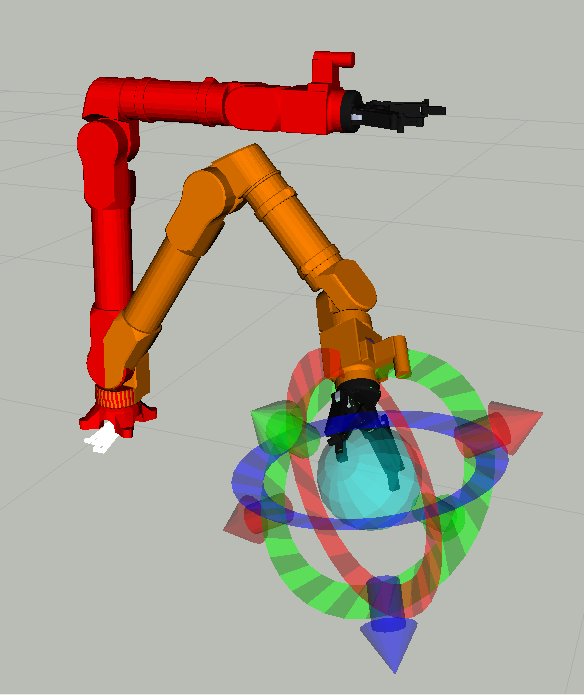
\includegraphics[scale=0.5]{Figures/ovis_moveit_industrial_sim}
    \caption{Ovis simulé par le simulateur industriel}
    \label{fig:ovis_industrial_sim}
\end{figure}

Sur la figure \ref{fig:ovis_industrial_sim}, on voit la position actuelle simulée (rouge), la position à atteindre simulée (orange) ainsi que le marqueur interactif (sphère cyan). Toutefois, on remarque que les joints de la pince robotique ne sont pas contrôlés (blanc). Ceci est dû à la lacune suivante du simulateur industriel. Le simulateur industriel est conçu pour un seul manipulateur, il n'émule donc pas plus d'un contrôleur logiciel. Les doigts de la pince ne sont pas localisés dans l'espace et se retrouvent affichée par défaut à la base du manipulateur.

\subsection{Simulation avec Gazebo}
En raison des lacunes que présente le simulateur industriel, il fut décidé que pour la suite du projet, il serait préférable de configurer la simulation Gazebo. Pour configurer la simulation Gazebo, il est possible d'utiliser le \emph{MoveIt Setup Assistant}, celui-ci génère un fichier URDF de base compatible avec Gazebo. Toutefois, ce fichier n'est pas modulaire et donc plus difficile à modifier et entretenir à l'avenir. Il fut donc décidé de continuer l'approche modulaire et d'étendre le contenu de la définition Xacro\footnote{\href{http://wiki.ros.org/xacro}{wiki.ros.org/xacro}} afin d'y inclure les paramètres spécifique à Gazebo tel que l'inertie, l'emplacement des capteurs de force et de la caméra du poignet. Il est aussi nécessaire d'ajouter le \emph{plugin} pour simuler le contrôleur logiciel du robot.

% \subsubsection{Abandon de la simulation Gazebo}
% Étant donné qu'il est complexe de modèliser le système et ne pouvant pas confirmer la validité de la simulation avec le bras réel, il fut décidé d'abandonner l'effort de simulation. Les efforts seront plutôt concentrés sur l'inter-connexion entre le logiciel et le matériel.

\subsection{Implémentation du contrôle linéaire}
La beauté de l'écosystème ROS est bien entendu sa communauté vouée à la recherche et au développement de la robotique. Il est souvent aisé de trouver une entité qui à dû traiter un problème identique ou similaire et qui publie sa solution librement. En cherchant une solution pour le déplacement linéaire d'un robot manipulateur, on a trouvé que le Tokyo Opensource Robotics Kyokai (TORK) avait déjà travaillé sur cette problématique. Leur solution \emph{jog\_control} étant librement accessible, il a donc suffit d'adapter le fichier de lancement de cette suite logicielle afin de la faire interagir avec le manipulateur.

\subsubsection{Contrôle du manipulateur à l'aide de la souris 3D}
\begin{figure}
    \centering
    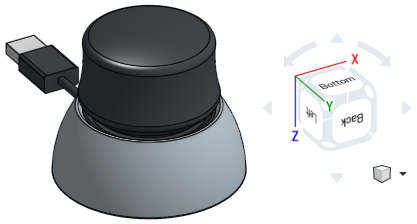
\includegraphics[width=0.65\textwidth]{Figures/spacemouse_axis_4.png}
    \caption{Le système d'axes de la souris 3D}
    \label{fig:spacemouse_axis}
\end{figure}

Le logiciel \emph{jog\_control} contenait déjà un exemple permettant de contrôler un manipulateur à l'aide d'une manette de jeux videos. L'exemple fut testé à l'aide d'une manette Xbox afin de valider qu'il était fonctionnel. Par la suite, l'adaptation avec la souris 3D fut entreprise. L'exemple étant écrit en python, le prototype d'adaptation pour le contrôle avec la souris 3D l'est aussi. Ayant en tête le projet actuel, ce travail fut effectué à la session A2019\footnote{\href{https://github.com/tork-a/jog_control/commit/b1b27c9a034a166a8e04d271c7839f4741c848b4}{github.com/tork-a/jog\_control@b1b27c9}}. Le prototype calcule d'abord une multiplication matricielle afin de passer des axes de la souris 3D tel que montrés à la figure \ref{fig:spacemouse_axis} vers le référentiel local à l'effecteur. 

% Après des essais plus exhaustif, il semblerait qu'il y ait une erreur de logique dans le prototype. Ce dernier permet les déplacement seulement vers la borne positive d'un axe, le problème semble se situer à la fonction du mode dominant. Celle-ci filtre le tableau des axes et conserve seulement la valeur la plus élevée.

La réécriture complète du logiciel fut débutée. Cette fois-ci, le logiciel est écrit en C++ afin d'augmenter la rapidité d'exécution. La réécriture comprend aussi un remodelage des différentes fonctions et variables membre de la classe. La réécriture ne fut pas sans heurt, la librairie ROS pour le C++ est plus complexe que celle pour python. Il fallut aussi trouver une librairie afin d'effectuer les calculs matriciels nécessaires pour le calcul des rotations, la librairie Armadillo\footcite{sanderson_armadillo_2016} fut sélectionné en raison de sa documentation exhaustive et de sa facilité d'intégration avec ROS. Quelques recherches ont été nécessaire afin de configurer avec succès l'éditeur \emph{Visual Studio Code}\footnote{\href{https://github.com/RoboGnome/VS_Code_ROS}{github.com/RoboGnome/VS\_Code\_ROS}} afin d'être en mesure de déverminer le nouveau code. 

Le fonctionnement général de l'algorithme est le suivant: 
\begin{enumerate}[nosep]
    \item Les valeurs des axes de la souris 3D sont reçus;
    \item La valeur de l'axe le plus significatif est retenue;
    \item Les axes sont transformés de manière à refléter le système d'axes au manipulateur;
    \item Les valeurs transformées sont publiées afin d'être exécutées par le contrôleur du bras robotique.
\end{enumerate}
% \todo[inline]{Ajouter quelques algorithmes des sous-fonctions. Au minimum, d'écrire l'idée générale du calcul.}

\subsection{Essais sur le manipulateur}
\subsubsection{Configuration de la communication contrôleur-ordinateur}
Le contrôleur Kinova nécessite une configuration de départ. Étant donné la nature de notre projet par rapport à ceux de la clientèle typique de Kinova, il fut difficile de trouver l'information afin de configurer correctement le contrôleur. Les problèmes rencontrés étaient les suivant: la version du logiciel\footnote{\href{https://www.kinovarobotics.com/sites/default/files/UG-008_KINOVA_Software_development_kit-User_guide_EN_R02\%20\%281\%29.pdf}{Kinova Development Center}} livrée avec les actuateurs n'était pas la plus récente malgré que le \emph{firmware} %logiciel interne
des composants fut mis à jour; la configuration réseau nécessite que le contrôleur ait une adresse MAC propre à lui, la procédure de configuration de l'adresse MAC n'était pas disponible en ligne, il fut nécessaire de contacter le support technique. Finalement, en suivant la procédure de configuration pour utiliser le contrôleur Kinova par le port réseau, le logiciel est maintenant capable de communiquer avec le contrôleur et les actuateurs. Toutefois, la connexion n'est possible que de pair à pair, il semble impossible d'utiliser un commutateur Ethernet \emph{managed} entre les deux appareils.

\subsubsection{Interface matériel logiciel}
Avant de procéder à essayer le logiciel, on doit connecter le logiciel au matériel. Pour ce faire, les options sont d'utiliser le pilote informatique %driver en français selon Google, ouach
fourni par la solution \emph{kinova\_ros} ou d'utiliser la solution développée par le club Walking Machine aussi de l'ÉTS. Il fut choisi d'essayer la solution développée par Kinova étant donné qu'à première vue celle-ci semblait plus près de la solution recherchée.

\subsubsection{Détection du contrôleur via le protocole USB}
Lors de la première tentative de connexion entre l'ordinateur portatif et le contrôleur Kinova, le contrôleur n'était pas détecté. Suite à plusieurs recherches, le problème est causé par l'algorithme qui régule la consommation d'énergie et qui gère le bus USB. Cet algorithme permet en condition d'utilisation régulière d'économiser l'énergie en mettant en veille un périphérique qui n'est pas utilisé. Le contrôleur Kinova n'étant pas un produit grand public, celui-ci ne réagit pas de la manière attendu par l'algorithme. Le port USB est donc mis en veille, la communication avec le contrôleur est donc impossible. La solution la plus simple est de désactiver la mise en veille automatique pour tous les ports USB\footnote{\url{https://askubuntu.com/a/1161074}}. Une solution plus élégante est de modifier le fichier *.udev mais le temps étant limité cette approche sera explorée seulement si un problème de consommation élevée est détecté\footnote{\url{https://askubuntu.com/a/525916}}.

\subsubsection{Essai du pilote informatique \emph{kinova\_ros} sur un ordinateur portable}
Afin d'essayer la solution fournie par Kinova, l'écriture d'un  fichier de lancement ainsi que d'un fichier de configuration est nécessaire. Le fichier écrit pour le bras Ovis est calqué de celui existant pour lancer un bras Jaco de Kinova. Il est nécessaire d'ajuster quelques paramètres et le fichier lance le pilote informatique afin d'établir la communication avec le bras Ovis.

\subsubsection{Modification du pilote informatique \emph{kinova\_ros} pour l'architecture \emph{aarch64}}
Le pilote informatique fourni par Kinova est compatible seulement avec un ordinateur de bureau régulier possédant habituellement l'architecture \emph{x32} ou \emph{x86}. La plateforme Markhor est contrôlée par l'ordinateur embarqué, celui-ci repose sur l'architecture \emph{aarch64}. Le pilote informatique fourni n'est pas compatible avec la solution matérielle utilisé cela pose problème. Suite à plusieurs recherches, un autre dépôt logiciel fourni par Kinova contient les fichiers compilés pour l'architecture visée. Il est donc nécessaire d'adapter le pilote informatique afin qu'il soit apte à localiser et référencer ces fichiers correctement lors de la compilation et l'exécution du logiciel. La solution à ce problème consiste à ajouter les fichiers précompilés (.so) dans un dossier au nom de l'architecture spécifique du Jetson soit : "aarch64-linux-gnu". Le fichier d'instructions au compilateur\footnote{\href{https://cmake.org}{CMake.org}} étant écrit de manière paramétrique, aucune modification ne fut nécessaire.
% \todo[inline]{Compiler et tester l'exécution du logiciel sur le Jetson}

\subsection{Intégration de la pince à la solution}\label{subsec:pince_gazebo}
%% Ajout du contrôleur, simulation du contrôleur avec Gazebo?
Grâce à l'initiative ROS-Industrial, la pince Robotiq utilisée vient avec un paquet logiciel ROS\footnote{\href{https://github.com/ros-industrial/robotiq}{github.com/ros-industrial/robotiq}}. Ceci réduit grandement la complexité d'intégration de la pince à la solution. Toutefois, ce paquet ne comporte pas de support pour la simulation dans Gazebo. La figure \ref{fig:robotiq_gazebo} montre les doigts de la pince Robotiq simulés qui se comportent de manière erratique suite à une collision légère, bien entendu ceci ne correspond pas au comportement réel de la pince.

\begin{figure}
    \centering
    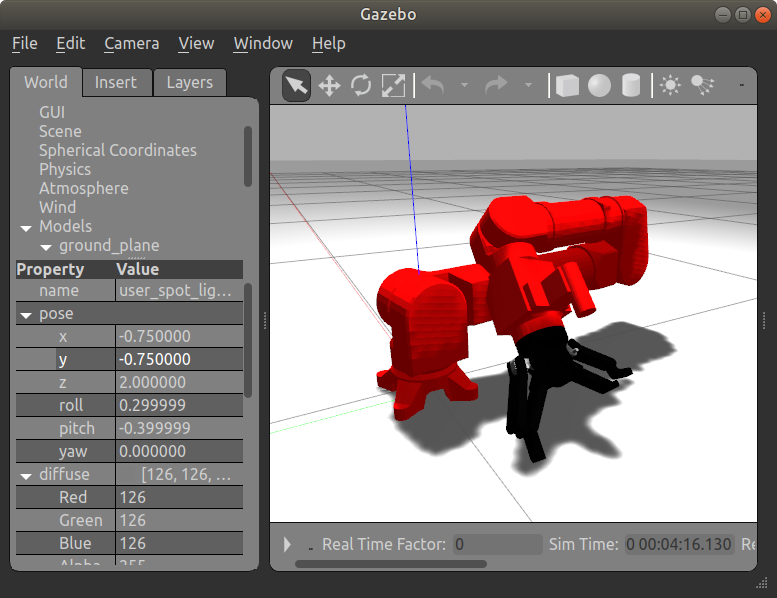
\includegraphics[width=\textwidth]{Figures/gazebo_ovis_sim.png}
    \caption{La pince Robotiq simulée avec Gazebo suite à une collision légère}
    \label{fig:robotiq_gazebo}
\end{figure}

Suite au développement de l'algorithme de contrôle du bras, il apparaît maintenant évident que le contrôle de la pince ne doit pas être intégré à celui-ci. Le contrôleur de la pince existant sera simplement lancé sur l'ordinateur embarqué de la plateforme mobile et le UI fera les appels nécessaires afin de contrôler manuellement l'ouverture/fermeture de la pince.